% Template for Cogsci submission with R Markdown

% Stuff changed from original Markdown PLOS Template
\documentclass[10pt, letterpaper]{article}

\usepackage{cogsci}
\usepackage{pslatex}
\usepackage{float}
\usepackage{caption}

% amsmath package, useful for mathematical formulas
\usepackage{amsmath}

% amssymb package, useful for mathematical symbols
\usepackage{amssymb}

% hyperref package, useful for hyperlinks
\usepackage{hyperref}

% graphicx package, useful for including eps and pdf graphics
% include graphics with the command \includegraphics
\usepackage{graphicx}

% Sweave(-like)
\usepackage{fancyvrb}
\DefineVerbatimEnvironment{Sinput}{Verbatim}{fontshape=sl}
\DefineVerbatimEnvironment{Soutput}{Verbatim}{}
\DefineVerbatimEnvironment{Scode}{Verbatim}{fontshape=sl}
\newenvironment{Schunk}{}{}
\DefineVerbatimEnvironment{Code}{Verbatim}{}
\DefineVerbatimEnvironment{CodeInput}{Verbatim}{fontshape=sl}
\DefineVerbatimEnvironment{CodeOutput}{Verbatim}{}
\newenvironment{CodeChunk}{}{}

% cite package, to clean up citations in the main text. Do not remove.
\usepackage{apacite}

% KM added 1/4/18 to allow control of blind submission


\usepackage{color}

% Use doublespacing - comment out for single spacing
%\usepackage{setspace}
%\doublespacing


% % Text layout
% \topmargin 0.0cm
% \oddsidemargin 0.5cm
% \evensidemargin 0.5cm
% \textwidth 16cm
% \textheight 21cm

\title{Selection of goal-consistent acoustic environments by adults and
preschool-aged children}



\newlength{\cslhangindent}
\setlength{\cslhangindent}{1.5em}
\newenvironment{CSLReferences}%
  {}%
  {\par}

\begin{document}

\maketitle

\begin{abstract}
Children are navigating a world with massive amounts of auditory input,
sometimes relevant while other times purely noise, and must somehow make
sense of it all. The early auditory environment is critical for speech
perception and recognition, auditory discrimination, and word learning,
all of which support language outcomes. What strategies do children use
to learn in noisy environments? One potential strategy is environmental
selection, which allows children to seek environments that align with
particular goals. In the current paper, we examined whether children and
adults make decisions about their environments by integrating auditory
information and goal-states. While 3- and 4-year olds struggle with
discrmininating the level of noise in noisy speech streams (and likely
do not use this information for environmental selection), 5-year-old
children and adults can. Further, we show initial evidence that they can
use this information to reason about acoustic environments that are
consistent with specific goals.

\textbf{Keywords:}
active learning; auditory discrimination; auditory noise; cognitive
development
\end{abstract}

\hypertarget{introduction}{%
\section{Introduction}\label{introduction}}

Children's auditory environment supports language development, but this
environment can also be noisy and chaotic. Acoustic noise is ubiquitous
and unavoidable, from sounds as low as a whisper (30dB) to as high as
crowded restaurants (90dB) (Erickson \& Newman, 2017). Children struggle
with speech perception and word recognition in noisy environments, and
often require signal-to-noise (SNR) levels of 5-7dB higher than adults
listening to the same stimulus (Bjorklund \& Harnishfeger, 1990; Klatte,
Bergström, \& Lachmann, 2013). Despite this, children manage to make
sense of such a noisy world.

More than 20 million children living in the United States are exposed to
dangerous noise levels daily, and 5 million of those children suffer
from noise-induced hearing loss as a result (Viet, Dellarco, Dearborn,
\& Neitzel, 2014). Unfortunately, children of color living in urban
regions are overrepresented in these numbers (Casey et al., 2017).
Chronic exposure to noise has been correlated with poorer reading
performance, reduced short term and episodic memory, and smaller
expressive vocabularies in elementary school children (Clark, Sörqvist,
\& others, 2012; Hygge, 2019; Riley \& McGregor, 2012). Yet despite
suboptimal conditions, language acquisition, cognitive development, and
full engagement with the environment is still possible, albeit more
difficult. What strategies do children use in these conditions?

One observation is that children's attention or discrimination abilities
may shift when faced with suboptimal auditory patterns, even if this
causes deleterious long- term outcomes. Cohen, Glass, \& Singer (1973)
measured the sound pressure levels in and around a noisy Manhattan
high-rise apartment complex where 8- and 9-year-old middle class
students lived. Auditory discrimination mediated the relationship
between reading comprehension/ability and auditory noise. Children
exposed to higher levels of auditory noise in the home filtered out
noise, but appeared to lose important information in the process.

Children might also learn to optimize their auditory environments to
successfully complete certain goals. For example, a child might find
that reading is best done in a library, not just because of its
convention (because libraries function as places to read/check out
books), but because it is a quiet space. Such a strategy might allow
children to exploit environmental variation in noise to maximize their
ability to learn in suboptimal or variable conditions. In the current
paper, we asked whether preschool children can reason about their
auditory environment and how it relates to specific goals.

Environmental selection of this type is a type of active learning, in
which an agent makes choices to shape its own learning. The dominant
approach to studying active learning has emphasized how learners
approach individual stimuli (e.g., Settles, 2009). When faced with
uncertainty, both human and machine systems can learn actively by
choosing new stimuli to query that are informative with respect to the
learner's current knowledge state (Castro et al., 2008). Infants, too,
have been shown to use active learning strategies (Ruggeri, Swaboda,
Sim, \& Gopnik, 2019; see Xu, 2019 for review).

Although most active learning research has focused on stimulus
selection, perhaps children and adults are engaging in active learning
by also making decisions about the environments in which they learn. In
practice, this behavior may present itself as moving to a different room
to study for an upcoming exam or playing in a room with other children
who seem to be having the kind of fun you desire. We might expect humans
to seek out environments that best support their goals, and observe this
strategy even in young children.

In the current paper, we took a first step towards investigating whether
children and adults actively select their auditory environment to
achieve their goals. We conducted two experiments with both children and
adults. Although our primary interest is whether and how children engage
in environmental selection, we also collected adult samples to offer
comparisons of how cognitively mature individuals might respond to these
tasks. To ensure that the stimuli we use can be discriminated by
children in our target ages, Experiments 1a and 1b investigate children
and adults' auditory discrimination of noise in long speech streams.
Experiments 2a and 2b then examine whether children and adults can
select auditory environments that match a goal.

\hypertarget{experiment-1a}{%
\section{Experiment 1a}\label{experiment-1a}}

Previous research has consistently shown that adults can discriminate
when two different sounds are at or below 5db apart, and children as
young as four perform similarly to adults in discriminating contrasts as
low as 5db (Jensen \& Neff, 1993). However, the stimuli commonly used to
measure auditory (or intensity) discrimination tend to be short tonal
bursts. These differ considerably from children's real-world auditory
experiences, which are not always transient and can reflect more
sustained noise. Additionally, noise exposure is not limited to
non-speech noise (e.g., white noise). Thus, in our first experiment, we
aimed to build on previous discrimination studies by creating a noise
discrimination and preference paradigm that used longer audio streams
(up to 25s) and naturalistic multi-talker noise.

\hypertarget{methods}{%
\subsection{Methods}\label{methods}}

\hypertarget{participants}{%
\subsubsection{Participants}\label{participants}}

A total of 40 adults (mean age = 27.68 years; 52.5\% Caucasian/White)
living in the United States at the time of test were recruited to
participate via the online platform Prolific. Testing was restricted to
a laptop, desktop, or tablet. All participants were fluent in English
and had no severe visual or cognitive impairments. For this reason, an
additional 6 participants were excluded from analysis. Informed consent
was collected from each participant before the experiment began.

\hypertarget{materials-and-procedure}{%
\subsubsection{Materials and Procedure}\label{materials-and-procedure}}

\begin{CodeChunk}
\begin{figure}[t]

{\centering 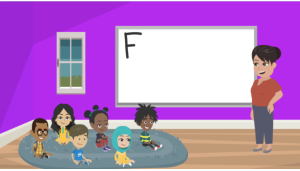
\includegraphics{figs/e1-stimuli-1} 

}

\caption[One of 10 animated classrooms participants viewed during the session]{One of 10 animated classrooms participants viewed during the session.}\label{fig:e1-stimuli}
\end{figure}
\end{CodeChunk}

Participants were told that they would watch 25s animated videos from
each of the ten classrooms in The Alphabet School, a fictional preschool
program in which each class learns one letter of the alphabet from A--J.
Classrooms were created with Vyond animation software. Each classroom
was depicted in the videos as having 5--6 preschool children and one
adult teacher with stereotypical male or female presentation. The wall
colors of each classroom identified which classroom participants were
viewing. In each video, the teacher would tell the students which letter
of the alphabet they would be learning, followed by three images on a
whiteboard of animals or objects that begin with that letter. Figure 1
illustrates one of the ten classrooms shown during the session.

Participants viewed two videos per trial, for a total of five trials.
Importantly, the classrooms differed in their signal-to-noise ratios
(SNR), which ranged from 5--25dB. Each teacher's speech was registered
at 65dB, and the background noise, a recording of live preschool
classrooms collected by the first author, were equalized on speech
subtracting any silence in the clips, and ranged from 35--60dB. The two
videos for each trial differed from each other in noise level by
5--25dB. At the end of each trial, participants indicated which
classroom was the louder of the two. To ensure that participants
understood the referent of the question, we also asked at the end of the
experiment whether the term ``louder'' referred to the loudness of the
speaker or the loudness of the background noise. Additionally, to reduce
participant inattention in the data, we included two attention check
questions and excluded participants who answered at least one question
incorrectly. SNR levels of each classroom were counterbalanced across
trials and conditions.

\hypertarget{results-and-discussion}{%
\subsection{Results and Discussion}\label{results-and-discussion}}

\begin{CodeChunk}
\begin{figure}[t]

{\centering 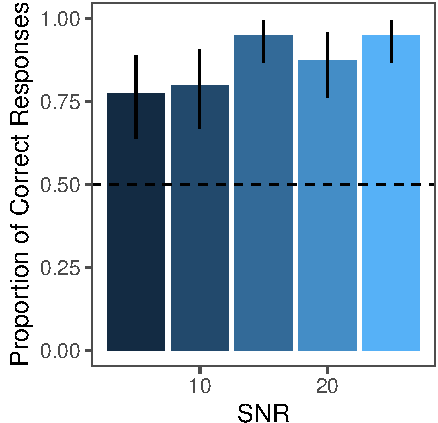
\includegraphics{figs/e1a-bar-1} 

}

\caption[Results from Experiment 1a]{Results from Experiment 1a. Proportion of correct responses across SNR levels from 5--25dB. Error bars show 95\% confidence intervals.}\label{fig:e1a-bar}
\end{figure}
\end{CodeChunk}

Given prior data, we expected that across SNR levels, adults would
correctly identify relative differences in the auditory environments
presented in this experiment (which served primarily as a comparison for
Experiment 1b with children). We preregistered {[}OSF link removed for
anonymous submission{]} a Bayesian mixed-effects logistic regression
predicting correct responding as a function of SNR, with a maximal
random effect structure (random slopes by SNR and a random intercept by
participant). SNR level was centered at 15 dB. In this and subsequent
models, we used default weakly informative priors (normal distributions
on coefficients with SD=2.5, scaled to predictor magnitudes).

On average, adults were above chance across all five SNR levels
(intercept: \(\beta\) = 2.15, 95\% Crl = {[}1.66 - 2.88{]}), and there
was a modest effect of SNR on performance (intercept: \(\beta\) = 0.08,
95\% Crl = {[}0.01 - 0.16{]}). Data are shown in Figure 2.

This finding is both a replication of previous studies which have found
similar performance levels in adults, as well as an extension that
revealed these findings hold even with more complex stimuli. These
results affirm adults' auditory discrimination skills are fully mature,
and that they possess the cognitive resources necessary to successfully
complete this task.

\hypertarget{experiment-1b}{%
\section{Experiment 1b}\label{experiment-1b}}

In Experiment 1b, we reran the same experiment with
3--5-year-old-children.

\hypertarget{methods-1}{%
\subsection{Methods}\label{methods-1}}

\hypertarget{participants-1}{%
\subsubsection{Participants}\label{participants-1}}

36 children (mean age = 4 years, 41.7\% Caucasian/White) completed the
same task as adults in Experiment 1a with a few notable differences. An
additional 7 children were ultimately excluded from analysis because
their caregivers indicated they heard English less than 75\% of the
time.

\hypertarget{materials-and-procedure-1}{%
\subsubsection{Materials and
Procedure}\label{materials-and-procedure-1}}

Children were tested synchronously over the Zoom platform by an
undergraduate research assistant. The researcher first collected
informed consent from the caregiver, who was often present but
instructed not to engage during the session, followed by assent from the
child. Children whose caregivers pointed to the computer screen or
provided answers during the session were excluded from analysis. Due to
the age range of interest, the experiment was presented strictly though
images and videos, and the research assistant verbally explained each
slide to the children. Between trials, children were rewarded with
virtual gold stars, which also served to pace the experiment and to
maintain engagement. Finally, children were not asked to identify the
referent of the question.

\hypertarget{results-and-discussion-1}{%
\subsection{Results and Discussion}\label{results-and-discussion-1}}

\begin{CodeChunk}
\begin{figure}[t]

{\centering 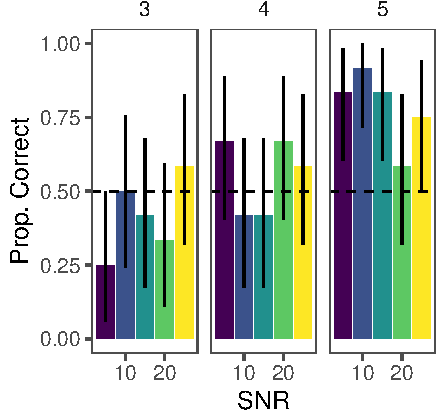
\includegraphics{figs/e1b-bar-1} 

}

\caption[Experiment 1b]{Experiment 1b. Proportion of correct responses across SNR levels from 5--25dB. Error bars show 95\% confidence intervals.}\label{fig:e1b-bar}
\end{figure}
\end{CodeChunk}

We anticipated that, while the strength of the effect would increase
with age, all children would correctly identify relative differences in
SNRs from 10--25dB, and that only three-year-old children would be
unable to correctly identify this difference at 5dB. We ran the same
Bayesian logistic regression presented in Experiment 1a, but added age
(centered at the mean) as a main effect. Figure 3 demonstrates a
similar, though weaker, pattern of auditory discrimination skills in
preschool children. In the aggregate, 3--5-year-old children showed some
discrimination ability on the current paradigm (intercept : \(\beta\) =
-4.52, Crl = {[}-6.77 - -2.42{]}), but independent of SNR (intercept :
\(\beta\) = 0.14, Crl = {[}-0.14 - 0.42{]}).

Age played a larger role in children's performance than we anticipated.
To explore this effect, we binned the data by the child's age in years
{[}3;0-3;11, 4;0-4;11, and 5;0-5;11 years{]} and reran the same
analysis. Older children were more likely to correctly discriminate
auditory signals than younger children (intercept : \(\beta\) = -3.14,
Crl = {[}-4.94 - -1.47{]}).

Our findings differed from prior results in that only 5 year olds
appeared to be robustly above chance in discrimination. There are
several possible reasons for this disparity. First, as described
earlier, this task is much more challenging than prior rapid
discrimination tasks: it requires assessing the level of noise in a
video, remembering it, and comparing it to another over the course of
almost a minute. Additionally, the type of stimuli presented here
differs from the tonal bursts or other non-speech sounds used in earlier
work.

\hypertarget{experiment-2a}{%
\section{Experiment 2a}\label{experiment-2a}}

If 5-year-old participants can successfully discriminate between sound
pressure levels, can they then use this information to reason about
which goals are most appropriate in these environments? In our next set
of experiments, we assessed this hypothesis. Participants watched a
video of a third-person character with several goals and were asked to
select the environment in which he should complete these goals. As in
Experiment 1, we began by assessing performance in a convenience sample
of adults.

\hypertarget{methods-2}{%
\subsection{Methods}\label{methods-2}}

\hypertarget{participants-2}{%
\subsubsection{Participants}\label{participants-2}}

128 adults (mean age = 27.82 years; 69.5\% Caucasian/White) living in
the United States at the time of test were recruited to participate via
the online platform, Prolific. An additional 19 participants were
excluded from analysis for failing one or more of the attention checks.
Testing was restricted to a laptop, desktop, or tablet. All participants
were fluent in English and had no severe visual or cognitive
impairments. Informed consent was collected from each participant before
the experiment began.

\hypertarget{materials-and-procedure-2}{%
\subsubsection{Materials and
Procedure}\label{materials-and-procedure-2}}

Participants were introduced to a preschool-aged character named Ryan
with eight goals to complete throughout the experiment: (1) to read a
book, (2) to build a tower out of blocks, (3) to learn the letters of
the alphabet, (4) to paint a picture, (5) to dance to his favorite
music, (6) to learn a new language called Zerpie, (7) to talk to a
friend, and (8) to eat lunch. All activities had relatively simple
explanations with the exception of (6). For this trial, participants
were told that Ryan's new neighbor, Logan, speaks a rare language called
Zerpie, a language he doesn't speak. Ryan wants to learn Zerpie so he
can communicate with Logan.

In each of the eight trials, participants watched a video in which Ryan
stood in between two closed doors labeled ``A'' and ``B,'' respectively.
Before the video began, participants were told to watch and listen
carefully to decide which of the two rooms Ryan should go to in order to
complete his goal.

As in Experiment 1, we manipulated the sound level of each room, but
removed any classroom stimuli, including the teacher, and only depicted
one child opening and standing in front of each door. As such,
participants did not have access to any visual information about the
room, and could only rely on auditory information, as well as any
information provided by the character who opened the door. Each
character's voice was equalized to 65dB and, unlike in Experiment 1, all
characters shared the same voice. All characters except Ryan were
preschool girls but differed in appearance. The same background noise in
Experiment 1 was used for the current experiment, and the difference in
SNR between the two rooms was 5--25dB.

During the video, each character would open their respective door
beginning with Room A. The character in Room A always said, ``You can
{[}goal{]} in this room,'' while the character in Room B always said,
``Or you can {[}goal{]} in this room.'' While the room on the left was
always labeled ``A'' and the room on the right was always labeled ``B,''
the characters from and sound levels of each room, as well as goal order
were counterbalanced across conditions.

For each trial, participants were told which goal Ryan wanted to
complete and were asked to select the room that he should complete his
goal. After making a selection, they were then asked to briefly explain
their choice. Responses for the quieter room (relative to the other and
based on the actual sound pressure level) were given a 1, while
responses for the louder room were given a 0.

\hypertarget{results-and-discussion-2}{%
\subsection{Results and Discussion}\label{results-and-discussion-2}}

\begin{CodeChunk}
\begin{figure}[t]

{\centering 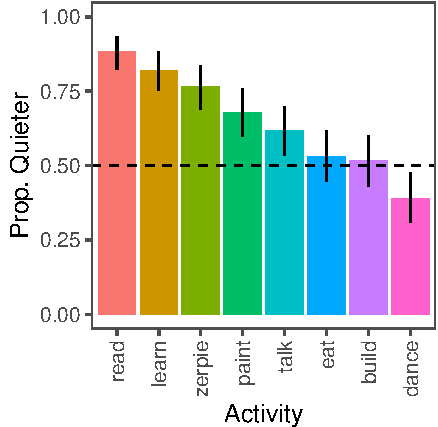
\includegraphics{figs/e2a-bar-1} 

}

\caption[Experiment 2a]{Experiment 2a. Proportion of participants selecting the quiet room based on activity, with activities sorted by response level.}\label{fig:e2a-bar}
\end{figure}
\end{CodeChunk}

We expected that adults would select the quieter room when the goal was
(1) to read a book, (2) to learn the new language called Zerpie, and (3)
to learn the letters of the alphabet, but would be more likely to select
the louder room when the goal was (1) to dance to his favorite music,
(2) to talk to a friend, and (3) to build a tower out of blocks.
Additionally, we expected participants to have no sound level preference
for (1) eating lunch and (2) painting a picture. This is because the
latter two activities might be more ambiguous in the degree to which a
relatively quieter or louder environment supports or hinders the goal.

As in Experiments 1a and 1b, we preregistered {[}OSF link removed for
anonymous submission{]} a Bayesian mixed-effects logistic regression
predicting environmental preference as a function of activity type.
Figure 4 depicts adult participants' preferences for quieter
environments based on the chosen activity. Coefficients for the read,
learn, Zerpie, paint, and dance activities all had 95\% credible
intervals that did not overlap with zero. Interestingly, only for the
dance activity did adults choose the louder room more than 50\% of the
time, likely reflecting some ambivalence about whether someone might
want to, e.g., eat in a loud room.

In sum, these findings suggests adults can reason about the match
between acoustic environments and activity goals.

\hypertarget{experiment-2b}{%
\section{Experiment 2b}\label{experiment-2b}}

In the next next study, we asked about whether children could also
evaluate the match between acoustic environments and activity goals.
Following the results of Experiment 1b, we conducted this experiment
with 5-year-olds only.

\hypertarget{methods-3}{%
\subsection{Methods}\label{methods-3}}

\hypertarget{participants-3}{%
\subsubsection{Participants}\label{participants-3}}

30 5-year-old children (69.5\% Caucasian/White) completed a truncated
version of Experiment 2a to both prevent testing fatigue and to maximize
any response differences based on the presented goals.

We tested children on the Zoom platform and also recruited a small group
of children at a local preschool. The in-person testing was conducted
with both caregiver consent and participant assent. As with the online
testing, participants were included only if they heard English at home
at least 75\% of the time and had no known cognitive, visual, or
neurological impairments, which led to an exclusion of an additional 8
children.

\hypertarget{materials-and-procedure-3}{%
\subsubsection{Materials and
Procedure}\label{materials-and-procedure-3}}

We tested children on the four activities with the widest differences
observed in Experiment 2a: (1) to read a book, (2) to learn the letters
of the alphabet, (3) to build a tower out of blocks, and (4) to dance to
music, for a total of four trials. Additionally, participants in this
experiment were only shown videos in which the two rooms had SNR
differences of 25dB because there were no differences in performance
across SNR levels in Experiment 1b.

Rooms and characters depicted in the videos remained consistent with
Experiment 2a, with one exception: the room labels, ``A'' and ``B,''
were replaced with one black circle for Room 1 and two black circles for
Room 2. This change was implemented after finding that several
participants in the pilot study seemed to favor the letter A over B, and
because these letter labels may interfere with responses when the goal
is to learn the letters of the alphabet. Black circle labels, on the
other hand, are more abstract and may reduce this bias. As done
previously, the characters, sound pressure levels, and goal order were
counterbalanced across conditions.

Whether testing online or in-person, participants were shown the same
set of videos and a research assistant (for online testing) or the first
author (for in-person testing) verbally explained each slide and video
to participants. After watching each video, participants were asked to
select the room Ryan should complete his goal and to briefly explain
their response. As in Experiment 2a, responses for the quieter room
(relative to the other and based on the actual sound pressure level)
were given a 1, while responses for the louder room were given a 0.

\hypertarget{results-and-discussion-3}{%
\subsection{Results and Discussion}\label{results-and-discussion-3}}

\begin{CodeChunk}
\begin{figure}[t]

{\centering 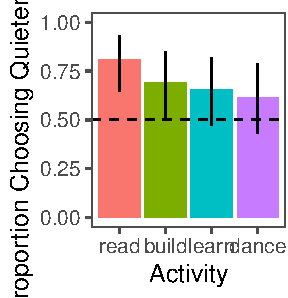
\includegraphics{figs/2b-bar-1} 

}

\caption[Experiment 2b]{Experiment 2b. Proportion of participants selecting the quieter room by activity.}\label{fig:2b-bar}
\end{figure}
\end{CodeChunk}

We expected to see a similar, though weaker, response pattern as adult
participants in Experiment 2a. Figure 5 depicts children's preferences
for quieter environments based on the chosen activity. We ran the same
logistic regression as in Experiment 2a. Children were more likely than
chance to select the quieter room for book reading (which was set to the
intercept: \(\beta\) = 1.56, Crl = {[}0.49 - 3{]}), but credible
intervals for the other activities overlapped zero, suggesting that they
could not individually be differentiated from those for the read
activity. Overall, children appeared to have a preference for the
quieter room across activities.

As an exploratory analysis, we asked whether the inclusion of other
activity predictors as a whole improved model fit by using bridge
sampling to compare between models with and without activity as a
predictor. This comparison revealed a Bayes Factor of 27.64 in favor of
the activity model, suggesting that as a whole these predictors did
substantially improve model fit and hence children showed some
sensitivity to goal in their room selections, despite their bias for the
quieter room.

\hypertarget{general-discussion}{%
\section{General Discussion}\label{general-discussion}}

We asked here whether adults and children can reason about how acoustic
noise changes the environment. We found that both 5-year-old children
and adults could discriminate noise levels differing by 5dB in long-form
auditory stimuli. On the other hand, 3- and 4-year-old children were
unable to do so. We then asked whether 5-year-olds and adults would
reason about which acoustic environments best matched a particular
activity goal. Adults showed clear and graded sensitivity, choosing
quieter environments for reading and learning and louder environments
for dancing. Five-year-olds were more likely to select the quieter room
overall but showed initial evidence that they differentiated between
activities as well.

In other research, children in the age ranges we studied show evidence
that they learn actively (Ruggeri, Swaboda, Sim, \& Gopnik, 2019; Xu,
2019), pursue ways to reduce uncertainty when faced with a possible
reward (Feldstein \& Witryol, 1971), and search for additional
information on a particular topic when their intuitive theories are less
informative (Wang, Yang, Macias, \& Bonawitz, 2021). Yet we found that
younger children struggled even to differentiate environments with
different levels of noise, and even 5-year-olds showed only modest
sensitivity to the congruence between acoustic environments and goals.
Each of these tasks may have been challenging for children for reasons
unrelated to their sensitivity to the underlying constructs, however.
The discrimination task required encoding and comparing noise levels
across two different 25s videos, which might have been challenging for
reasons of attention and memory. And the environmental selection task
required noticing that the rooms differed in noise levels and encoding
their noise levels as well as associating different noise levels with
particular activities. Thus, in future work we intend to explore simpler
and more naturalistic paradigms for evaluating children's environmental
selection abilities.

There are several further limitations that point the way towards new
experiments. First, our research relied on convenience samples and so
our specific estimates are not broadly generalizable to other
populations. Second, the paradigm used third-party scenarios where
participants assisted someone else with achieving certain goals; it is
still unknown whether children would make similar decisions if they
themselves were given goals to complete. Finally, there is a possibility
that familiarity influenced participants' environmental preferences.
Future work should explore novel activities where participants cannot
rely on their current knowledge about which auditory environments are
most optimal for each activity.

By understanding the strategies children use to learn in noisy auditory
environments, we might offer better solutions for those exposed to
chronic noise, thereby mitigating some of its negative effects. Such
mitigation is becoming more and more critical as cities become more
populated (bringing construction with it) and auditory noise becomes
even more unavoidable. Future studies will need to (1) explore the
developmental trajectory of environmental selection, and (2) examine the
boundaries of environmental selection by probing these questions with
other goals and in other contexts (e.g.~first-person settings).
Investigating how children learn in noise will ultimately bring us
closer to understanding how children can thrive across a wide range of
environments.

\hypertarget{acknowledgements}{%
\section{Acknowledgements}\label{acknowledgements}}

Removed for anonymous submission.

\hypertarget{references}{%
\section{References}\label{references}}

\setlength{\parindent}{-0.1in} 
\setlength{\leftskip}{0.125in}

\noindent

\hypertarget{refs}{}
\begin{CSLReferences}{1}{0}
\leavevmode\hypertarget{ref-bjorklund1990}{}%
Bjorklund, D. F., \& Harnishfeger, K. K. (1990). The resources construct
in cognitive development: Diverse sources of evidence and a theory of
inefficient inhibition. \emph{Developmental Review}, \emph{10}(1),
48--71.

\leavevmode\hypertarget{ref-casey2017}{}%
Casey, J. A., Morello-Frosch, R., Mennitt, D. J., Fristrup, K., Ogburn,
E. L., \& James, P. (2017). Race/ethnicity, socioeconomic status,
residential segregation, and spatial variation in noise exposure in the
contiguous united states. \emph{Environmental Health Perspectives},
\emph{125}(7), 077017.

\leavevmode\hypertarget{ref-castro2008}{}%
Castro, R. M., Kalish, C., Nowak, R., Qian, R., Rogers, T., \& Zhu, X.
(2008). Human active learning. In \emph{Advances in neural information
processing systems} (pp. 241--248). Citeseer.

\leavevmode\hypertarget{ref-clark20123}{}%
Clark, C., Sörqvist, P., \& others. (2012). A 3 year update on the
influence of noise on performance and behavior. \emph{Noise and Health},
\emph{14}(61), 292.

\leavevmode\hypertarget{ref-cohen1973}{}%
Cohen, S., Glass, D. C., \& Singer, J. E. (1973). Apartment noise,
auditory discrimination, and reading ability in children. \emph{Journal
of Experimental Social Psychology}, \emph{9}(5), 407--422.

\leavevmode\hypertarget{ref-erickson2017}{}%
Erickson, L. C., \& Newman, R. S. (2017). Influences of background noise
on infants and children. \emph{Current Directions in Psychological
Science}, \emph{26}(5), 451--457.

\leavevmode\hypertarget{ref-feldstein1971}{}%
Feldstein, J. H., \& Witryol, S. L. (1971). The incentive value of
uncertainty reduction for children. \emph{Child Development}, 793--804.

\leavevmode\hypertarget{ref-hygge2019}{}%
Hygge, S. (2019). Noise and cognition in children.

\leavevmode\hypertarget{ref-jensen1993}{}%
Jensen, J. K., \& Neff, D. L. (1993). Development of basic auditory
discrimination in preschool children. \emph{Psychological Science},
\emph{4}(2), 104--107.

\leavevmode\hypertarget{ref-klatte2013}{}%
Klatte, M., Bergström, K., \& Lachmann, T. (2013). Does noise affect
learning? A short review on noise effects on cognitive performance in
children. \emph{Frontiers in Psychology}, \emph{4}, 578.

\leavevmode\hypertarget{ref-riley2012}{}%
Riley, K. G., \& McGregor, K. K. (2012). Noise hampers children's
expressive word learning.

\leavevmode\hypertarget{ref-ruggeri2019}{}%
Ruggeri, A., Swaboda, N., Sim, Z. L., \& Gopnik, A. (2019). Shake it
baby, but only when needed: Preschoolers adapt their exploratory
strategies to the information structure of the task. \emph{Cognition},
\emph{193}, 104013.

\leavevmode\hypertarget{ref-settles2009}{}%
Settles, B. (2009). Active learning literature survey.

\leavevmode\hypertarget{ref-viet2014}{}%
Viet, S. M., Dellarco, M., Dearborn, D. G., \& Neitzel, R. (2014).
Assessment of noise exposure to children: Considerations for the
national children's study. \emph{Journal of Pregnancy and Child Health},
\emph{1}(1).

\leavevmode\hypertarget{ref-wang2021}{}%
Wang, J., Yang, Y., Macias, C., \& Bonawitz, E. (2021). Children with
more uncertainty in their intuitive theories seek domain-relevant
information. \emph{Psychological Science}, \emph{32}(7), 1147--1156.

\leavevmode\hypertarget{ref-xu2019}{}%
Xu, F. (2019). Towards a rational constructivist theory of cognitive
development. \emph{Psychological Review}, \emph{126}(6), 841.

\end{CSLReferences}

\bibliographystyle{apacite}


\end{document}
